\documentclass{article}
\usepackage{amsmath}
\usepackage{tikz}
\usepackage{hyperref}
\usetikzlibrary{positioning}
\newcommand\abs[1]{\left|#1\right|}

\begin{document}

\title{%
  Introduction to Graph Theory \\
  \large by Richard Trudeau \\
   Ch. 3 Solutions}
   \author{Tyler Bailey}
\maketitle

\begin{enumerate}

	\item[1] Prove the following statements:
	
	\begin{enumerate}
		\item[a] If 3 edges were added to the graph in Figure 63a, then at least 2 of the new edges will be adjacent.
		\item[b] Every graph with $v = 5$ and $e = 3$ has at least two adjacent edges.
		\item[c] If $v$ is an odd number, then every graph with $v$ vertices and $\frac{1}{2}(v + 1)$ edges has at least two adjacent edges.
	\end{enumerate}
	
	\textbf{Solution:}
	\begin{enumerate}
		\item[a] This is a straightforward application of the pigeonhole principle. If we add one edge, we connect two vertices. If we add another vertex it will either touch an existing vertex (and we are done) or not. If not, then we now have 4 vertices connected, none of which have adjacent edges, and one isolated vertex. For the final edge, no matter how we attach it, it must be adjacent to at least one other edge.
		\item[b] We proved this in item $a$ because we did not utilize the fact that Figure 63a was $C_5$.
		\item[c] This follows by the same pigeonhole argument as the previous two items. If we attach $\frac{1}{2}(v - 1)$ edges, we either have adjacent edges already, or we don't. If we don't, then we have connected a single isolated vertex and a final edge to add. Therefore, any connection will create two adjacent edges.
	\end{enumerate}
	
	\item[2] Prove that in Figure 58, graph a) is planar, and graphs b) and c) are non-planar.
	
	\textbf{Solution:}
		\begin{enumerate}
			\item[a] This graph is isomorphic to the following planar graph:
			
				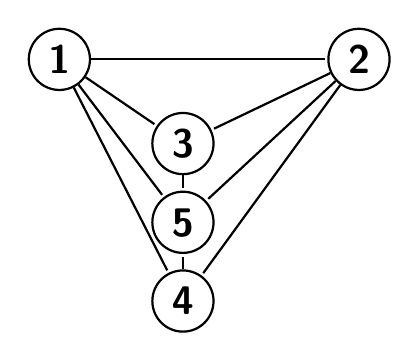
\begin{tikzpicture}[shorten >=1pt,auto,node distance=3cm,
                    thick,main node/.style={circle,draw,font=\sffamily\Large\bfseries}]
                    	\node[main node] (1) {1};
                    	\node[main node] (2) [right=3cm of 1] {2};
                    	\node[main node] (3) [below right=0.5cm and 1cm of 1] {3};
                    	\node[main node] (5) [below right=1.5cm and 1cm of 1] {5};
					\node[main node] (4) [below right=2.5cm and 1cm of 1] {4};

                    \path[every node/.style={font=\sffamily\small}]
             		(1)	edge node [left] {} (2)
                    		edge node [left] {} (3)
                    		edge node [left] {} (4)
						edge node [left] {} (5)
                 	(2)	edge node [right] {} (3)
                 		edge node [right] {} (4)
                 		edge node [right] {} (5)
                 	(3)	edge node [right] {} (5)
					(4)	edge node [right] {} (5);

				\end{tikzpicture}
			\item[b] This is a supergraph of $UG$.
			\item[c] $K_7$ is a supergraph of $K_5$.
		\end{enumerate}
	\item[3] Find a graph $G$ such that $every$ expansion of $G$ is also a supergraph of $G$.
	
	\textbf{Solution:} Take the path graph with two vertices, $P_2$.
	
	\item[4 - 5] Omitted, answers in book.
	
	\item[6] Draw a nonplanar graph whose complement is nonplanar.
	
	\textbf{Solution:} Take the graph which is $K_5$ and $\overline{UG}$ together. It is nonplanar because $K_5$ is, and the complement contains $UG$ as a subgraph, so it is nonplanar as well.
	
	\item[7] Prove the ``Petersen graph" is nonplanar.
	
		\textbf{Solution}: Number the graph starting at 1 at the outer apex going clockwise, then starting at 6 in the inner apex going clockwise.
		
		\begin{tikzpicture}[shorten >=1pt,auto,node distance=3cm, thick,main node/.style={circle,draw,font=\sffamily\Large\bfseries}]
			\node[main node] (1) [below left=2cm and 1.75cm of 2] {1};
			\node[main node] (2) {2};
			\node[main node] (3) [below=4cm of 2] {3};
			\node[main node] (4) [right=8cm of 2] {4};
			\node[main node] (7) [below right=.25cm and 1cm of 2] {7};
			\node[main node] (8) [right=4cm of 2] {8};
			\node[main node] (6) [below right=2.5cm and 2cm of 8] {6};
			\node[main node] (5) [below=4cm of 8] {5};
			\node[main node] (9) [below=4cm of 4] {9};
			\node[main node] (10) [below=2.5cm of 8] {10};
			\path[every node/.style={font=\sffamily\small}]
				(1)	edge node [left] {} (2)
                		edge node [left] {} (5)
                	(2)	edge node [right] {} (3)
                		edge node [right] {} (1)
               		edge node [right] {} (7)
				(4)	edge node [right] {} (5)
					edge node [right] {} (3)
					edge node [right] {} (9)
				(6)	edge node [right] {} (9)
				(7)	edge node [right] {} (9)
				(8)	edge node [right] {} (3)
                		edge node [right] {} (10)
               		edge node [right] {} (6)
               	(10)	edge node [right] {} (5);
		\end{tikzpicture}
		
		From this we can see that nodes 1, 7, 10, and 6 were expanded from $UG$.
		
	\item[8] Omitted for size.
	
	\item[9] Prove: if $H$ is an expansion of $G$ then $v_G + e_H = v_H + e_G$.
	
	\textbf{Solution}: If $H$ is an expansion of $G$ then we can derive $H$ from $G$ by successively expanding it. Start with $H$ = $G$. Then, of course, $v_G + e_H = v_H + e_G$. But each expansion increases $v_H$ by 1 and also $e_H$ by one, so the equation is always balanced.

	\item[10] Prove: if $H$ and $J$ are expansions of $G$G then $v_H + e_J = V_J + e_H$.
	
	\textbf{Solution}: This follows from the previous problem. Add $v_G + e_H = v_H + e_G$ and $v_J + e_G = v_G + e_J$, and cancel the $G$ terms.
	
	\item[11] Find all integers $v$ for which $\overline{C_v}$ is nonplanar. Prove that your answer is correct.
	
	\textbf{Solution}: The book shows that $\overline{C_7}$ is nonplanar. Additionally, for all $n > 7$, $\overline{C_n}$ has a subgraph isomorphic to $\overline{C_7}$. Label $\overline{C_n}$ starting at the top with 1 and increasing going clockwise. Form a subgraph using vertices $(1, 3, 5, 8, 2, 4, 7)$ and erase the appropriate edges to see it is isomorphic to $C_7$.
	\item[12] Use the pigeonhole principle to prove that there are at least two red maples in the United States having the same number of leaves.
	
	\textbf{Solution} This appears to be false as written (at least without additional assumptions). Counterexample: It is conceivable that there are only two trees, one with 0 leaves and one with 1 leaf.

	\item[13] Prove the following statements:
		\begin{enumerate}
			\item[a] Except for $UG$ itself, no expansion of $UG$ is also a supergraph of $UG$.
			\item[b] Except for $K_5$ itself, no expansion of $K_5$ is also a supergraph of $K_5$.
		\end{enumerate}

	\textbf{Solution}: 
		\begin{enumerate}
			\item[a] Suppose there was such a proper supergraph, and that it has a single vertex expanded. Then, for any selection of 6 vertices we can make, there are two cases to consider.
				\begin{enumerate}
					\item[Case 1]: We chose 6 vertices, none of which is an expanded vertex of degree 2. In this case, we have $v = 6$ and $e = 8$, which cannot be isomorphic to $UG$.
					\item[Case 2]: We chose 6 vertices, at least one of which is a vertex of degree 2, which means it cannot be isomorphic to $UG$.		
				\end{enumerate}
				In cases where there are more than one expansions made, the cases are similar, but in the first case we end up with $e \leq 8$.
				Therefore, no such supergraph exists.
			\item[b] Omitted. Similar argument to above.
		\end{enumerate}
	\item[14] Let $S$ be the set of all expansions of supergraphs of $UG$ or $K_5$, and let T be the set of all supergraphs of expansions of $UG$ or $K_5$. Prove that $T$ is $not$ a subset of $S$ and therefore $S \neq T$, by finding a supergraph of an expansion of $K_5$ that is not also an expansion of a supergraph of $K_5$.

	\textbf{Solution}: Expand an inner edge of $K_5$, and then create a new vertex and connect the new vertex to the expanded inner edge. This is not achievable as an expansion of a supergraph, because we cannot connect the new expansion to the new vertex in the set $S$ by the order of operations (first apply supergraph, then apply expansion).
	
	\item[15] Isomorphism is ``transitive", that is, if $G \cong H$ and $H \cong J$, then $G \cong J$. This enables us to prove the following theorem.
	
	\textbf{Theorem}: If $H$ is planar and $G \cong H$, then $G$ is planar too.
	
	Use this fact to devise new proofs that the pairs of graphs in Figures 46, 51, 54, and 55 are not isomorphic.
	
	\textbf{Solution}:
		\begin{enumerate}
			\item[46] Clearly LHS is planar. RHS is isomorphic to $UG$ so $LHS \not\cong RHS$.
			\item[51] Clearly LHS is planar. RHS is isomorphic to $UG$ so $LHS \not\cong RHS$.
			\item[54] Clearly RHS is planar. LHS has subgraph isomorphic to $UG$, so LHS is nonplanar. Therefore $LHS \not\cong RHS$.
			\item[55] Clearly LHS is planar. RHS is a supergraph of an expansion of $UG$. Therefore RHS is nonplanar so $LHS \not\cong RHS$.
		\end{enumerate}
		
	\item[16] Prove that the graphs in Figure 89 are planar.
	
	\textbf{Solution} Figure b) is isomorphic to Figure 50 RHS.
	
	\item[17, 18 - 20] In Figures 91 - 93, decide whether each graph is planar or nonplanar and then prove that your choice is correct.
	
	\textbf{Solution:} Omitted / Answers in Book.
\end{enumerate}

\end{document}